\documentclass[10pt,a4paper]{report}
\usepackage[latin1]{inputenc}
\usepackage{amsmath}
\usepackage{amsfonts}
\usepackage{amssymb}
\usepackage{graphicx}
\usepackage{listings}
\usepackage{enumitem}
\usepackage{amsmath}
\usepackage{mathtools}

\graphicspath{ {testing/images/} }

\author{Brock Smedley}
\title{CS325 Assignment 1}

\lstset{frame=tb,
	aboveskip=3mm,
	belowskip=3mm,
	showstringspaces=false,
	columns=flexible,
	basicstyle={\small\ttfamily},
	numbers=none,
	breaklines=true,
	breakatwhitespace=true,
	tabsize=4
}

\begin{document}
	\maketitle
	
	\section*{1}
	Assume we have a merge sort function called $mergesort(a)$ which takes an array $a$ and returns the sorted version of $a$.
	\\
	
	First we sort S using mergesort (which is O(nlogn)).
	The algorithm then adds the first and last elements of the array. If their sum equals x, then we return true. 
	
	If the sum is less than x, then we remove the first element (we need to add a marginally larger number).
	
	If the sum is greater than x, then we remove the last element and add back the first element if it had been previously removed (we may need the previous first element which we previously eliminated to make a valid sum with the new end number).
	
	We recursively call a helper function with the updated S (either with the first element removed; or the last element removed and the first element re-added).
	This way, we're guaranteed to hone in on the best candidates for making the sum.
	
	I believe the worst case running time for this algorithm is $O(3/2n)$ where X is a constant less than $3/2$. The only way one could incur this many operations is for the algorithm to make n comparisons, half of which result in the first element being re-appended while the last element is deleted, effectively keeping S the same size (unless the first element hasn't been previously deleted). Because S is sorted, the algorithm is only able to do this once for every other element (worst-case) because if we have to re-add the first element, we can be guaranteed that our sum was too high. If we only ever get sums that are too low, we'll finish the operation in n iterations. If we only ever get sums that are too high, we'll do the same. But if we go back and forth between low and high at every iteration, then every other iteration leaves the size the same as the last iteration. As a result, in this case the size of S decreases by 1 every other iteration. So in this special case, we add n/2 operations to our base count of n iterations, which we know has to happen to cover all possible pairs with the first element.
	\\
	Regardless of how much computing time this algorithm takes, it is still linear, and less than nlogn, which is the running time of a merge sort. Therefore, we simply take O(nlogn) to be our final running time, which we can call $\Theta$(nlogn) because we know that our sub-algorithm is linear and the runtime depends most on the merge sort, the running time of which is easy to predict. Our bounds c1 and c2 would be defined by the minimum and maximum runtime of our sub-algorithm: $\Omega$(1)*(nlogn) and O(3/2)*(logn).
	\\
	\newpage
	The following code implements the algorithm in Python:
	
	\begin{lstlisting}
# python 2.7 code
def hasSum(S,x):
	S = mergesort(S)
	return checkSum(S,x,-1,-1)


def checkSum(S,x,h):
	first = S[0]
	last = S[-1]
	_sum = first + last
	
	# base case 1: out of elements
	if (len(S) == 1):
		return False
	
	# base case 2: found a pair
	if (_sum == x):
		return True
	elif (_sum < x):
		h = S.pop(0)
	elif (_sum > x):
		if (h != -1):
			S.insert(0,h)
		h = -1
	return checkSum(S,x,h)
		
	\end{lstlisting}
	
	
	\newpage
	\section*{2}
	\begin{enumerate}[label=(\alph*)]
		\item f is O(g).
		
		Because the functions are polynomials of different degrees, we can guarantee that the one with the highest degree will always grow faster (the highest degree belonging to g(n)). g is an upper limit on f so f is O(g).
		
		\item f is $\Omega$(g).
		
		After n=1 (where we will set $n_0$), f(n) grows faster than g(n). Therefore g is a lower bound on f and f is $\Omega$(g).
		
		\item f is O(g).
		
		f(n) never exceeds g(n); g is an upper limit on f, so f must be O(g).
		
		\item f is $\Omega$(g).
		
		Because these are exponential functions with the same power, we know that the function with the higher base will always grow faster. Therefore, g is a lower limit on f and f is $\Omega$(g).
		
		\item f is O(g).
		
		Because these are exponential functions with the same base, we know that the function with the highest power will grow faster, which is g. g is an upper limit on f, so f is O(g).
		
		\item f is O(g).
		
		We know that the factorial function eventually grows faster than any exponential function. Therefore we know that g is an upper bound on f, so f is O(g).
	\end{enumerate}

	
	\newpage
	\section*{3}
	\begin{enumerate}[label=(\alph*)]
		\item 
		$f_1(n)$ = O(g)
		
		$f_2(n)$ = O(g)
		
		\begin{equation*}
		\begin{rcases}
		f_1(n) \le c_1 * g(n) \\
		f_2(n) \le c_2 * g(n)
		\end{rcases}
		\text{ By definition of big-O }
		\end{equation*}
		
		$f_1(n) + f_2(n) \le c_1 * g(n) + c_2 * g(n)$
		
		$f_1(n) + f_2(n) \le (c_1 + c_2) * g(n)$
		\\
		
		Because the value of constants can be ignored, we can combine the constants to get the following:
		\\
		
		$f_1(n) + f_2(n) \le (c) * g(n) = O(g(n))$ (by definition of big-O) $_\square$
		\\
		
		\item
		Counter-example:
		$f(n) = log(n)$\\
		$g_1(n) = log(n^2)$\\
		$g_2(n) = n^2$
		
		For $g_1(n)$ to be $\Theta(g_2(n))$ it must be $\Omega(g_2(n))$ and $O(g_2(n))$. $g_1$ cannot be $\Omega(g(n))$ so therefore it cannot be $\Theta(g(n)) _\square$

		
		
	\end{enumerate}


	\newpage
	\section*{5}
	\begin{enumerate}
		\item[(a,b)] 
		\begin{lstlisting}
			# hw1 - insertion sort
			# Brock Smedley
			
			from random import *
			import time
			
			
			def isort(dArr):
			for i in range(1,len(dArr)):
			focus = dArr[i]
			
			# shift other elements (> focus)
			k = i - 1
			while (k >= 0 and focus < dArr[k]):
			dArr[k + 1] = dArr[k]
			k = k - 1
			
			dArr[k + 1] = focus
			
			return dArr
			
			
			# generates random data to be sorted
			def readData(n):
			arr = []
			for i in range(n):
			arr.append(randint(0,10000))
			
			return arr
			
			
			def main():
			# generate data
			sizes = [1000, 2000, 5000, 10000, 25000, 50000]
			for s in sizes:
			data = readData(s)
			
			# sort it
			startTime = time.time()
			data = isort(data)
			endTime = time.time()
			
			print ("running time %s items: %s s" % (s, (endTime - startTime)))
			
			
			main()
			
			# Thank you to Mohit Kumra			
		\end{lstlisting}

		\newpage
		\begin{lstlisting}
			# hw1 - merge sort
			# Brock Smedley
			
			from random import *
			import time
			
			# receives array with indices representing two halves
			# a: start half1
			# b: end half1
			# c: end half2
			def merge(dArray, left, mid, right):
			x = mid - left + 1
			y = right - mid
			
			# temporary arrays; fill with data from dArray
			leftArr = []
			rightArr = []
			for i in range(x):
			leftArr.append(dArray[left + i])
			for j in range(y):
			rightArr.append(dArray[mid + 1 + j])
			
			# merge temporary arrays back into original array
			i = 0
			j = 0
			t = left
			
			while (i < x and j < y):
			if leftArr[i] <= rightArr[j]:
			dArray[t] = leftArr[i]
			i = i + 1
			else:
			dArray[t] = rightArr[j]
			j = j + 1
			t = t + 1
			
			# get rest of leftArr
			while (i < x):
			dArray[t] = leftArr[i]
			i = i + 1
			t = t + 1
			
			# get rest of rightArr
			while (j < y):
			dArray[t] = rightArr[j]
			j = j + 1
			t = t + 1
			
			
			# dArray: array of data to sort
			# left: index of left edge
			# right: "      " right ""
			# returns sorted array
			def mergesort(dArray, left, right):
			if (left < right):
			mid = (left + right) / 2
			
			# sort halves recursively
			mergesort(dArray, left, mid) # left half
			mergesort(dArray, mid + 1, right) # right half
			merge(dArray, left, mid, right) # merge sorted halves
			
			return dArray
			
			
			# generates random data to be sorted
			def readData(n):
			arr = []
			for i in range(n):
			arr.append(randint(0,10000))
			
			return arr
			
			
			
			def main():
			# generate data
			sizes = [1000, 2000, 5000, 10000, 25000, 50000]
			for s in sizes:
			data = readData(s)
			
			# sort it
			startTime = time.time()
			data = mergesort(data, 0, len(data)-1)
			endTime = time.time()
			
			print ("running time %s items: %s s" % (s, (endTime - startTime)))
			
			
			main()
			
			# Thank you to Mohit Kumra
		\end{lstlisting}
		
		\item[(c)]
		
		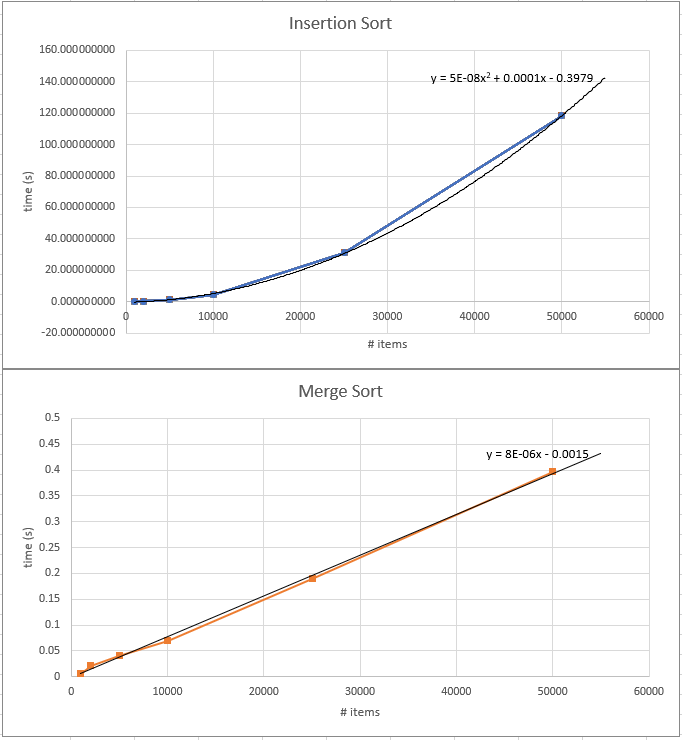
\includegraphics[scale=0.6]{sbs.png}
		
		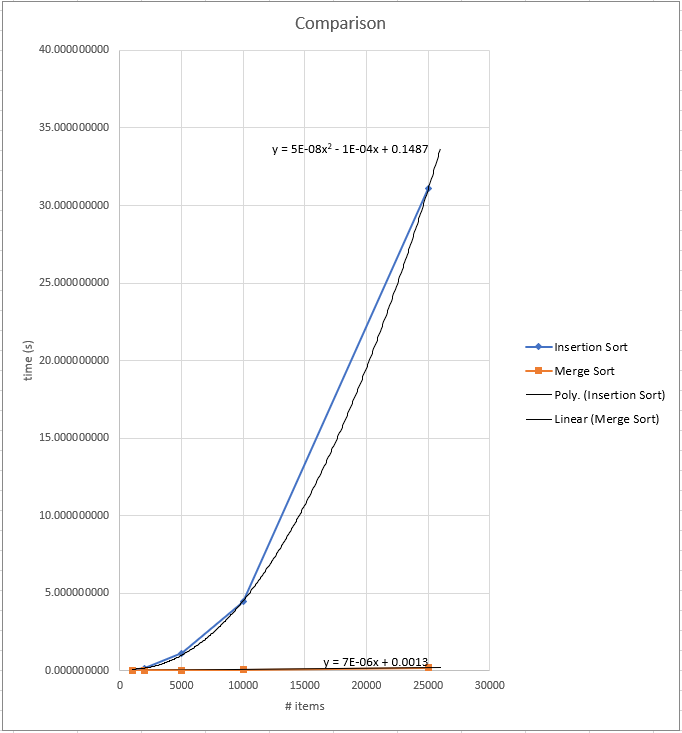
\includegraphics[scale=0.6]{overlay.png}
		
		The charts with individual graphs show the details of the data the best, but the overlaid graph very clearly illustrates the difference in running time.
		
		\item[(d)] Linear was the best fit for merge sort; it is $O(nlogn)$ so it makes sense for a trial with high numbers (50,000). You can see the logarithmic properties earlier in the curve but as n increases, it gets increasingly linear. As for insertion sort, it was clearly polynomial (to the second degree).
		
		\item[(e)] The average running times were similar to what I predicted they would be. Just by looking at the curve you can see how the algorithm works. I wasn't expecting such a long wait time for insertion sort with 50K elements, but it's not really surprising when you realize that insertion sort is a $O(n^2)$.
	\end{enumerate}
	
	
	
\end{document}